\chapter{Design}

\begin{longtabu} to \linewidth{@{}l l l X[j]@{}}
    Version &    Dato &    Ansvarlig &    Beskrivelse\\[-1ex]
    \midrule
    
\label{version_Systemark}
\end{longtabu}

\section{Indledning}
Formålet med design afsnittet er at beskrive hardwaren og softwaren for blodtryksmålersystemet. Systemet beskrives ved hjælp af udregninger, diagrammer, figurer og skitser som tydeligører, hvordan de forskellige delelementers funktionalitet er, samt hvilke tanker der ligger til grund for den endelige implementering (se afsnit \ref{Hardware implementering} for hardware og afsnit \ref{implementering} for software).

\section{Hardware arkitektur}
I følgende afsnit beskrives hvordan blodtryksmåler systemet og dets delkomponenters opbygning.
\\
\begin{figure}[H]
	\centering
	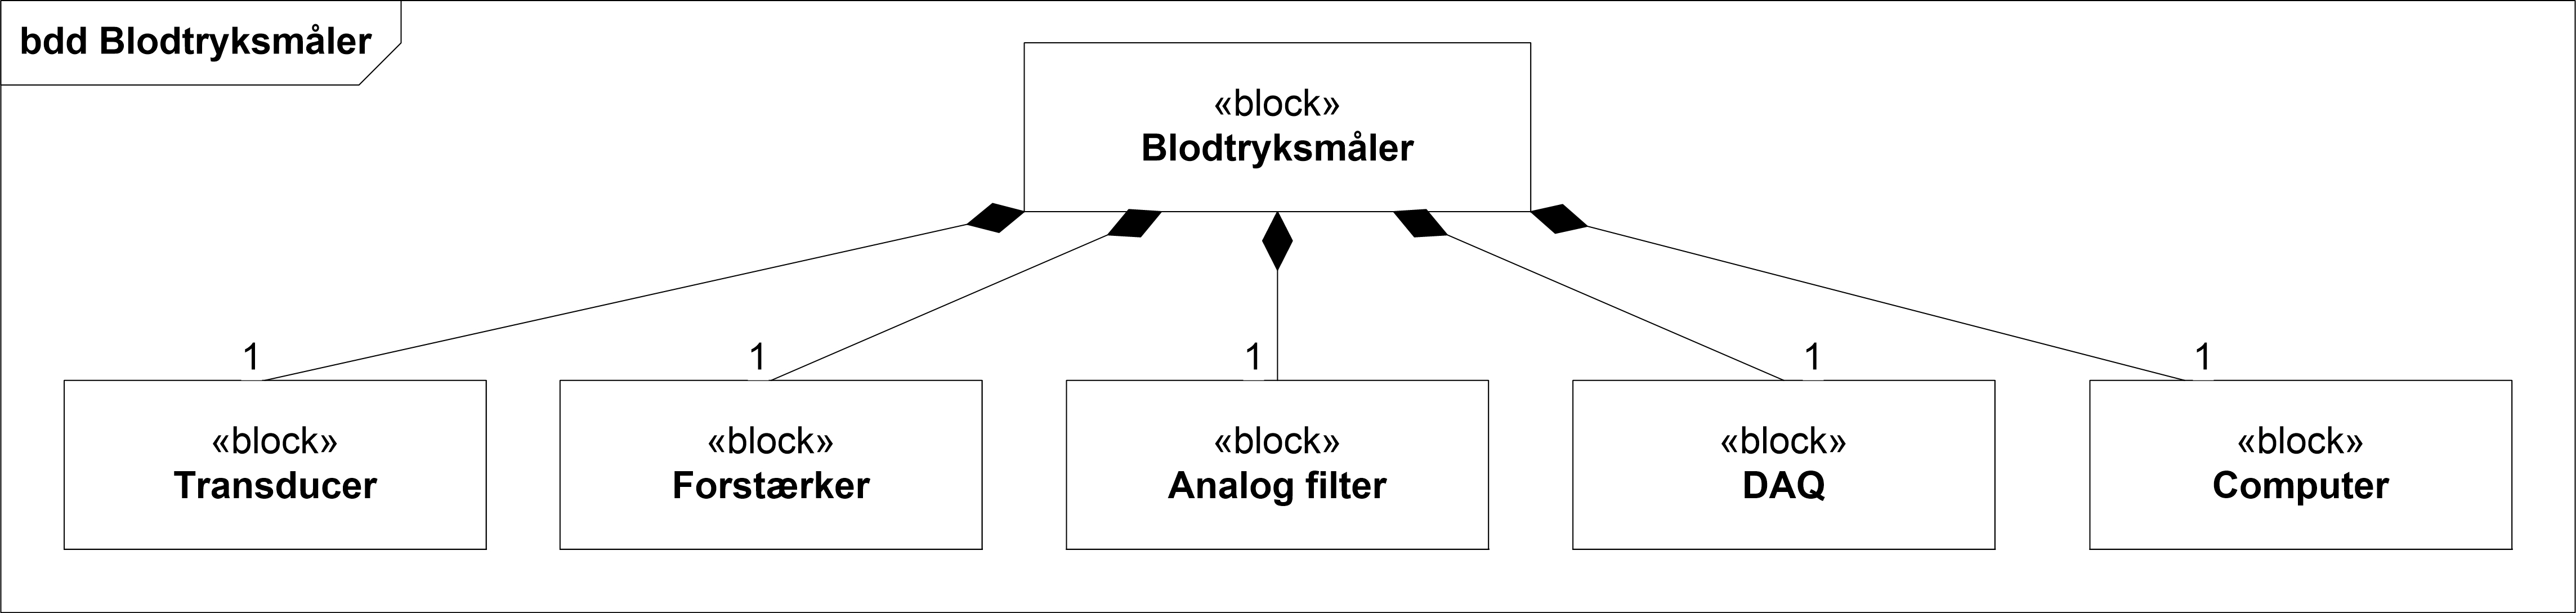
\includegraphics[width=1\textwidth]{Figurer/Hardware/BDD1}
	\caption{Blokdiagram for blodtryksmåler systemet.}
	\label{BDD blodtryksmaaler}
\end{figure}

Ud af blokdiagrammet, figur \ref{BDD blodtryksmaaler}, kan man se at blodtryksmåler systemet består af en transducer, en forstærker, et analogt filter, en DAQ og en computer.\\
\begin{figure}[H]
	\centering
	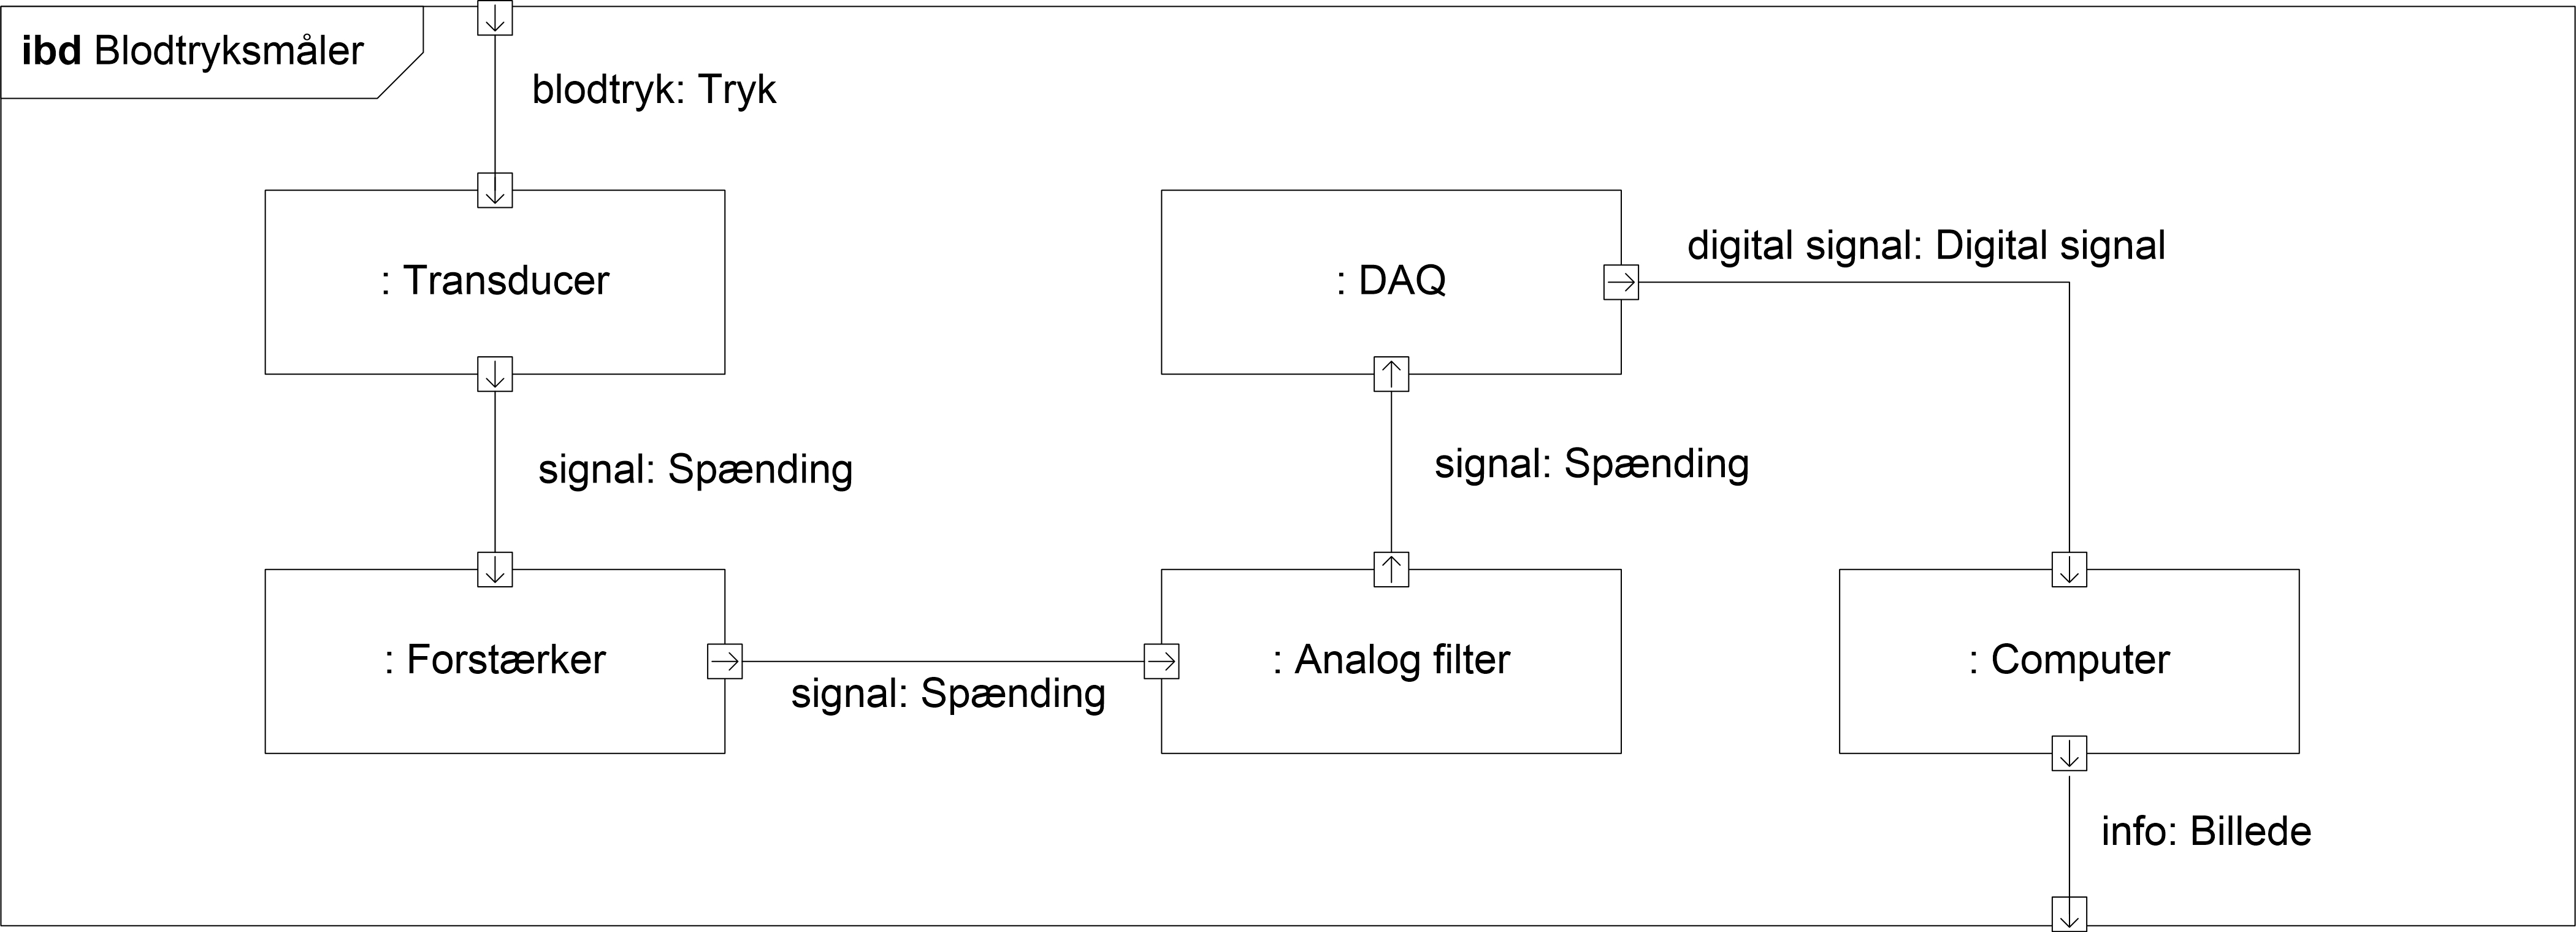
\includegraphics[width=1\textwidth]{Figurer/Hardware/IBD}
	\caption{Internt blok diagram for blodtryksmåler systemet.}
	\label{IBD blodtryksmaaler}
\end{figure}

Ud af det interne blok diagram, figur \ref{IBD blodtryksmaaler}, kan ses det at blodtrykket i form af det målte tryk kommer ind i transduceren. Transduceren som omformer det målte tryk til et spændingssignal, sender signalet vidre til forstærkeren. Fra forstærkeren sendes signalet over i det analoge filter og derfra ind i DAQ'en. Endeligt sendes det digitale signal fra DAQ'en over i en computer, der fortolker signalet som et billede, der vises til omverdenen.

\subsection{Design af forstærker}
Forstærkeren er designet med tanke på, at det er meget små spændinger der arbejdes med. Grundet dette, er en almindelig operationsforstærker fravalgt, da dens reelle indgangsimpedans ikke er for lav. En Instrumentationsforstærkers indgangsimpedans i den virkelige verden, er højere, og den kan dermed opfange meget små signaler, som f.eks. blodtryk, der opererer i millivolt..\\
Vejleder rådede herefter til at projektgruppen brugte instrumentationsforstærkeren INA114. Forstærkerens design er valgt ud fra instrumenteringsforstærkerens datasheet’s forslag, og kan ses på figur \ref{labelpic}.\\ 
\begin{figure}[H]
	\centering
	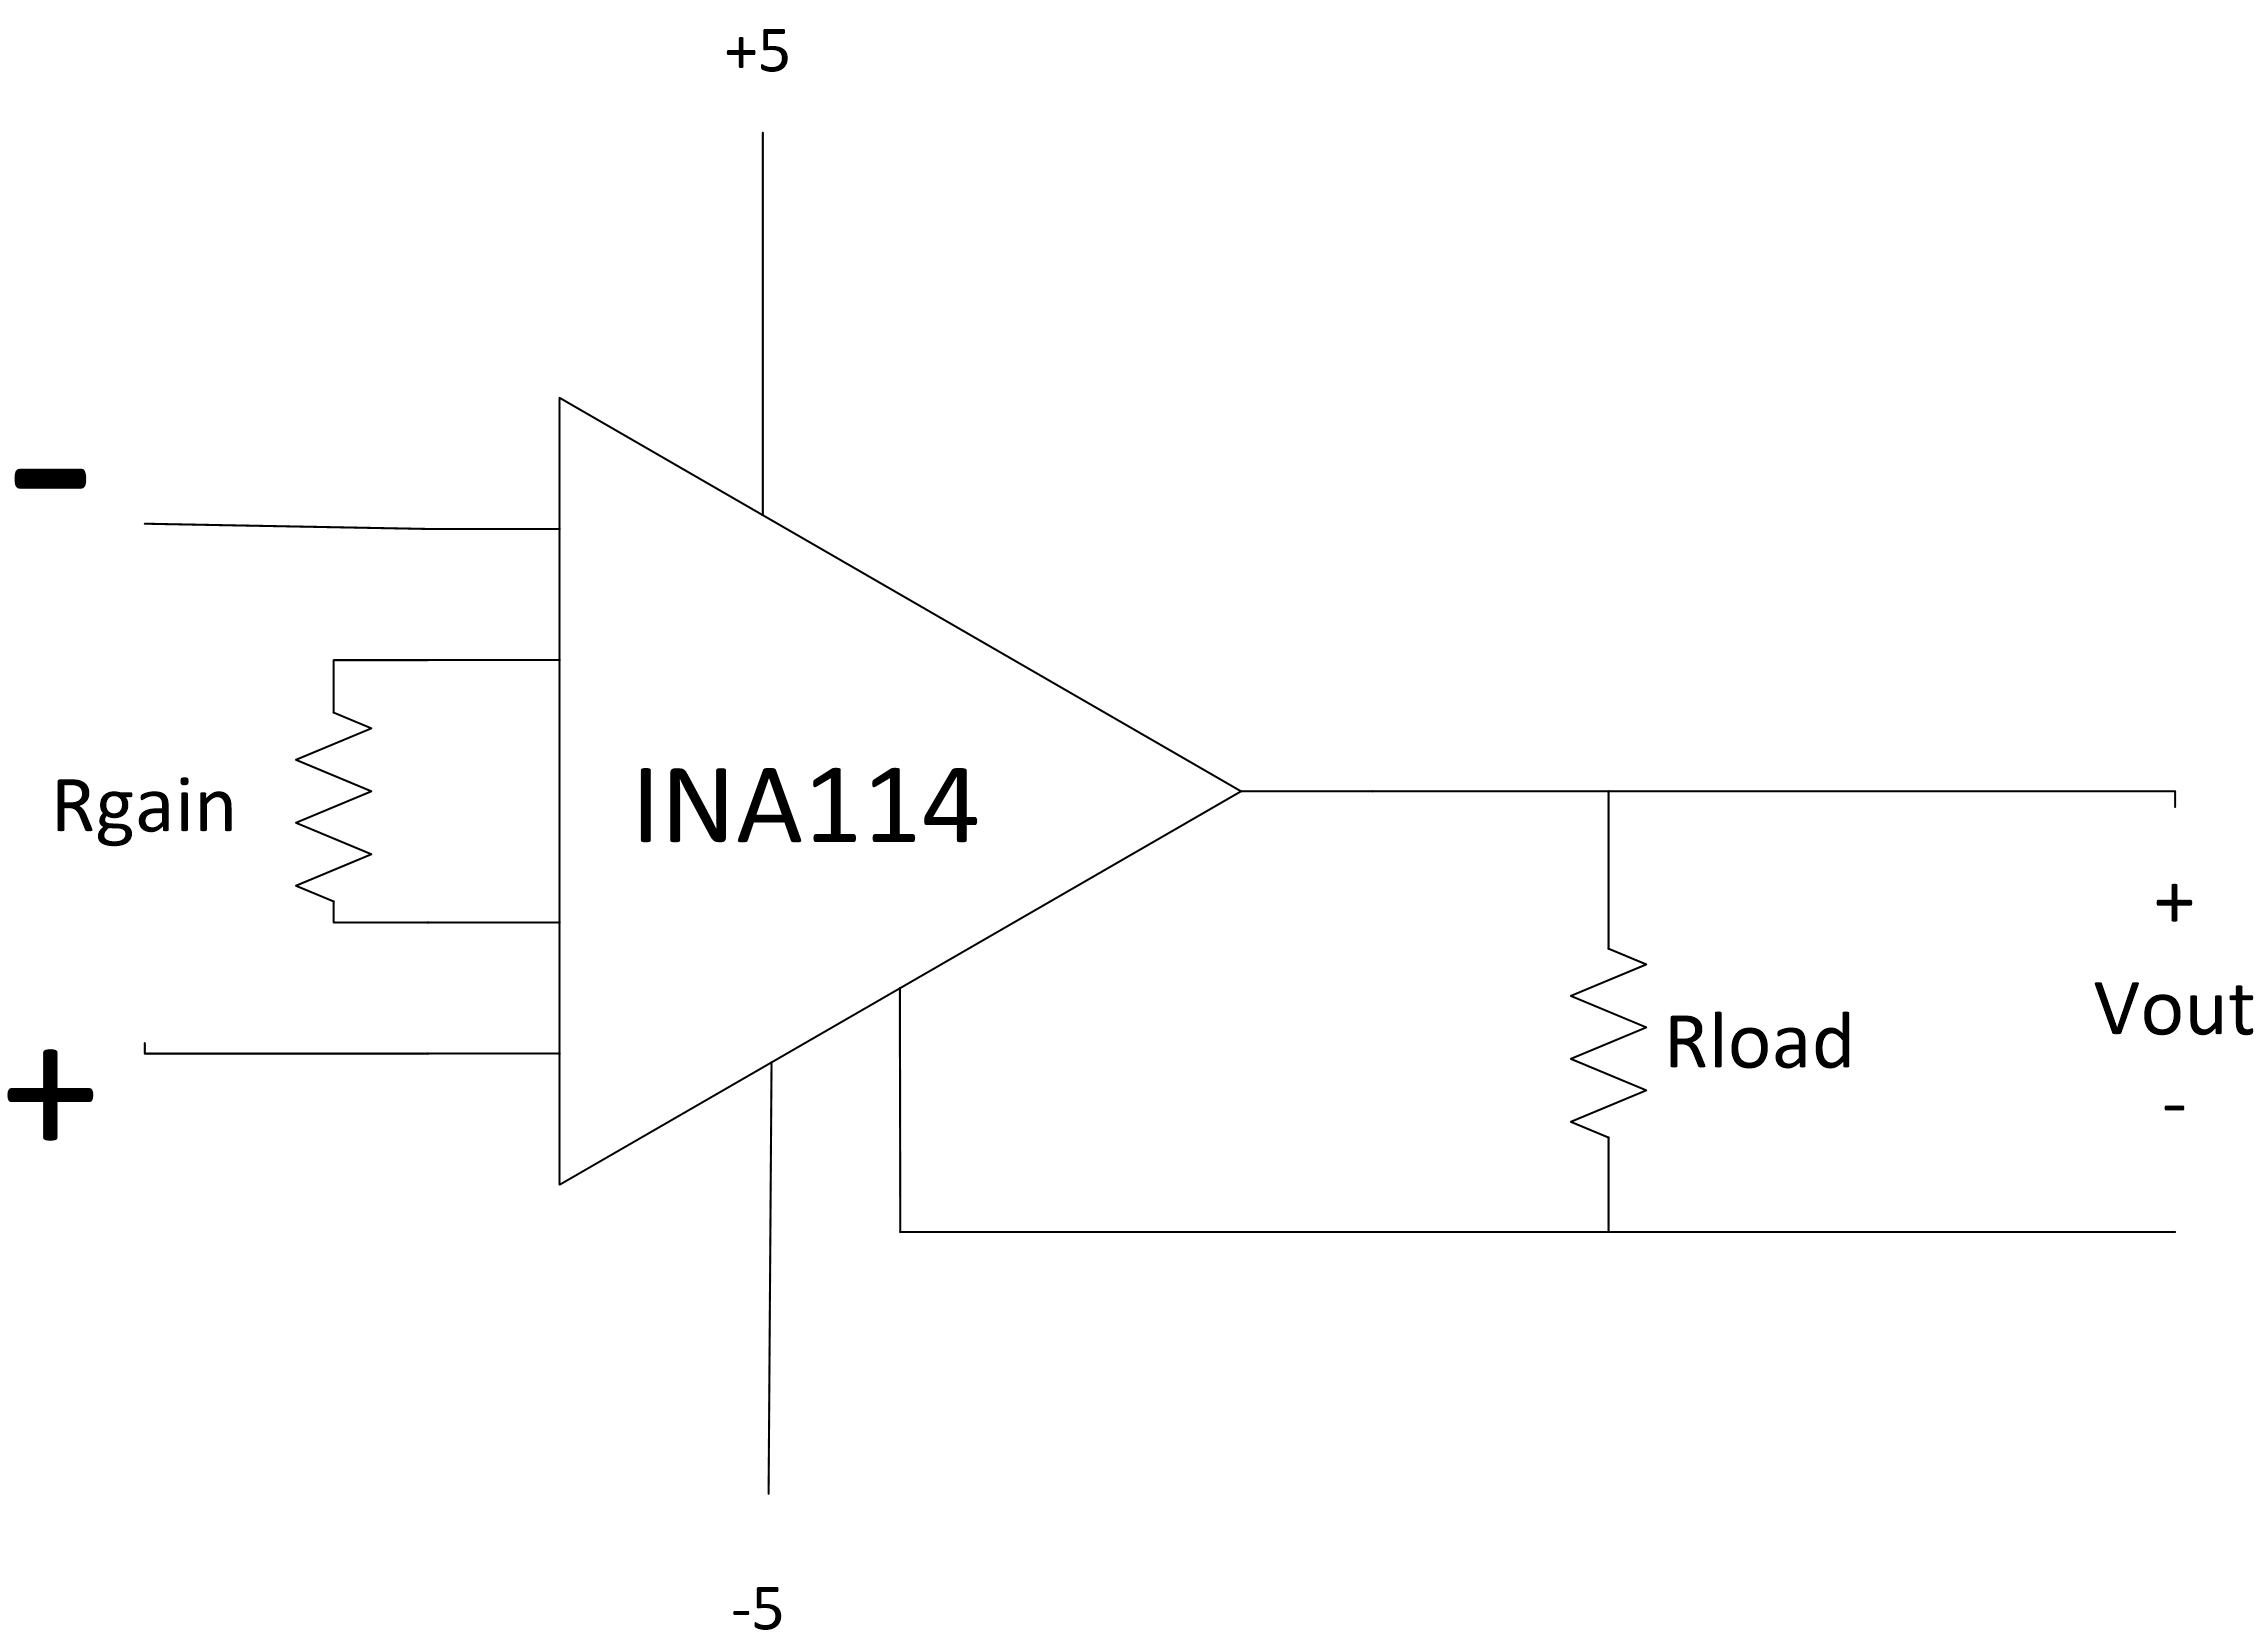
\includegraphics[width=0.6\textwidth]{Figurer/Hardware/Forstaerker}
	\caption{Der overordnede design af forstærkeren.}\label{labelpic}
\end{figure}



$R_{gain}$ er modstanden, som bestemmer, hvor meget forstærkning, instrumentationsforstærkeren skal give og $R_{load}$ er den belastning, der kommer efter kredsløbet. I dette tilfælde, er det, det analoge filter. For at finde $R_{gain}$’s størrelse, kræver det, at der vides, hvor meget forstærkning der er brug for. Dette findes, ved at bestemme den maksimale spænding, som transduceren kan give, i en blodtrykssituation. Dette regnestykke kan ses realiseret i ligning \ref{ligning1}:

\begin{align}
	VT_{max}=T_{max}\cdot V_{max}\cdot HG_{max}=\frac{\mu V}{V/mmHG}\cdot 5V\cdot 250mmHg=6,25mV
	\label{ligning1}
\end{align}

Spændingen ønskes at skaleres op til DAQ’ens dynamikområde, som ligger omkring 2,5V. Forstærkningsfaktoren udregnes ved simpel brøkregning, som ses på ligning \ref{ligning2}:

\begin{center}
	\begin{align}
		G=\frac{2,5}{6,25 \cdot 10^{-3}}=400
		\label{ligning2}
	\end{align}
\end{center}

INA114’s datasheet giver en ligning for udregning af forstærkning. Da forstærkningen er kendt, omskrives ligning \ref{ligning3} , så modstanden $R_{gain}$’s værdi i stedet bestemmes:\\


\begin{align}
	Gain=1+\frac{50k\Omega}{R_{gain}}\to G-1=\frac{50k\Omega}{R_{gain}}\to \frac{50kOhm}{G-1}=R_{gain}
	\label{ligning3}
\end{align}

Herefter kan den ohmske værdi af $R_{gain}$ bestemmes, hvilket sker i ligning \ref{ligning4}:

\begin{align}
	R_{gain}=\frac{50k\Omega}{400-1}=125,31 \Omega
	\label{ligning4}
\end{align}

\subsection{Design af analogfilter}
Filteret, som ses på figur \ref{fig:Filter}, skulle realiseres som et aktivt 2. ordens lavpasfilter af typen Sallen-Key med unity gain, med båndbredde på 50 Hz (se \ref{fig:Filter}). Desuden skulle filteret yderligere designes som et Butterworth filter med cut off frekvens på 50 Hz. C2 skulle vælges til at være 680 nF og gruppen fik desuden at vide, at R1 skulle være lig med R2. Operationsforstærkeren blev opgivet til at være af typen OP27.  

\begin{figure}[H]
	\centering
	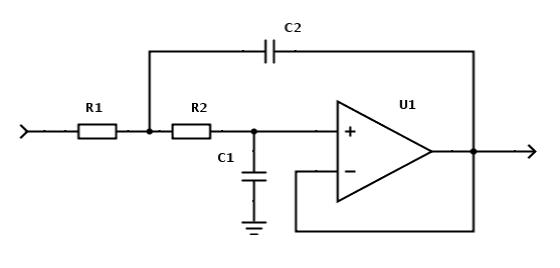
\includegraphics[width=1\textwidth]{Figurer/Hardware/FilterDesign}
	\caption{Unity gain 2. ordens Sallen-Key lavpas konfiguration}
	\label{fig:Filter}
\end{figure}

Et Sallen-Keyfilter har en dæmpningsfaktor på 0,7, fordi at der, i et Sallen-Key filter, er blevet prioriteret et fladt frkvensområde, frem for hurtig dæmpning. Gruppen brugte en hjemmeside\footnote{http://sim.okawa-denshi.jp/en/OPseikiLowkeisan.htm} som hjælpemiddel til at finde overføringsfunktionen for Sallen-Key lavpasfilteret. Denne ligning kan ses i ligning \ref{ligning5}:


\begin{align}
	\frac{V_{out}(S)}{V_{in}(S)}=\frac{\frac{1}{R_1C_1R_2C_2}}{s^2+s(\frac{1}{R_2C_2}+\frac{1}{R_1C_2})+\frac{1}{R_1C_1R_2C_2}}
	\label{ligning5}
\end{align}

Da det er blevet opgivet at $R1=R2$, kan overføringsfunktionen forkortes, som set på ligning \ref{ligning6}.

\begin{align}
\frac{V_{out}(s)}{V_{in}(s)}=\frac{\frac{1}{R^2C_{1}C_{2}}}{s^2+s(\frac{2}{RC_{2}})+\frac{1}{R^2C_{1}C_{2}}}
\label{ligning6}
\end{align}

Dernæst sammenlignes med standardformlen for overføringsfunktionen for et andet ordens filter på figur \ref{ligning7};

\begin{align}
\frac{V_{out}(s)}{V_{in}(s)} = \frac{\frac{1}{R^{2}C_{1} C_{2}}}{s^2+s(\frac{2}{RC_{2}})+\frac{1}{R^{2}C_{1}C_{2}}} = \frac{\omega_{0}^{2}}{s{2}+s(2\zeta\omega_{0})+\omega_{0}^{2}}
\label{ligning7}
\end{align}

Ud fra dette kan regnes komponentværdierne for R, idet vi har en opgivet værdi for $\frac{2}{RC_{2}}$, som vist på figur \ref{ligning8}

\begin{align}
\frac{2}{RC_{2}}=2\zeta\omega_{0}
\label{ligning8}
\end{align}

Gruppen brugte herefter MathCad til at isolere R, og herefter udregne værdien af denne. Dette kan ses på figur \ref{ligning9}
\begin{align}
\frac{2}{R\cdot680\cdot10^{-9}}=2\cdot0.7\cdot(50\cdot2\cdot\pi) solve, R \to \frac{250000}{17\cdot\pi}=6.687\times 10^3
\label{ligning9}
\end{align}

Dernæst kan komponentværdien for C1 udregnes, da gruppen nu havde en formel, men en ubekendt.


\begin{align*}
\frac{1}{R^2C_{1}C_{2}}=\omega_{0}^2
\label{ligning10}
\end{align*}	

Ved hjælp af MathCAD isoleres C1. 

\begin{align}
	\frac{1}{(6.687\times 10^{3})^{2}\cdot(680\cdot10^{-9})\cdot C_1}=(50\cdot 2\pi)^{2} solve, R \to 333,2\times 10^{-9}
\end{align}

Derved er komponentværdierne for kredsløbet fundet og de ses indskrevet på \ref{fig:Filter}. 

\begin{figure}[H]
	\centering
	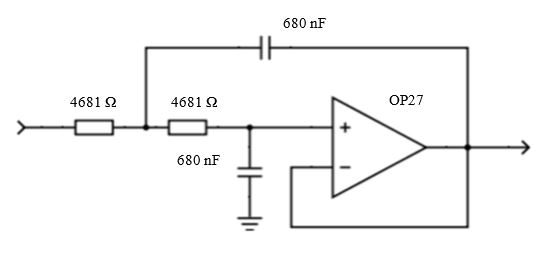
\includegraphics[width=1\textwidth]{Figurer/Hardware/FilterDesignMedKomponentvaerdier}
	\caption{Unity gain 2. ordens Sallen-Key lavpas konfiguration med indsatte komponentværdier.}
	\label{fig:Filter_K}
\end{figure}

For at underbygge gruppens teori omkring filteret, blev der ved hjælp af toolet ”Sallen-Key Low-pass Filter Design Tool”\footnote{http://sim.okawa-denshi.jp/en/OPseikiLowkeisan.htm} udarbejdet et bodeplot. Dette kan ses nedefor på figur \ref{fig:Bodeplot}. 

\begin{figure}[H]
	\centering
	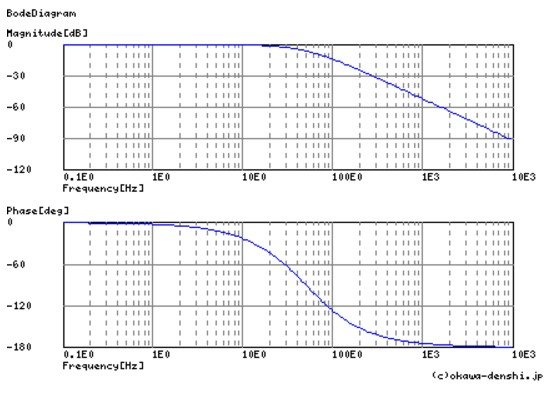
\includegraphics[width=1\textwidth]{Figurer/Hardware/Bodeplot}
	\caption[]{Bodeplot af overføringsfunktionen\footnotemark}
	\label{fig:Bodeplot}
\end{figure}
\footnotetext{\url{http://sim.okawa-denshi.jp/en/OPseikiLowkeisan.htm}}


\subsection{Grænseflader}

\begin{table}[H]
\centering
\small
\begin{tabular}{|l|l|l|l|l|}
\hline
\textbf{Navn} & \textbf{Input}  & \textbf{Output} & \textbf{Interval}                                                                   & \textbf{Beskrivelse}                                                                                                                                                                          \\ \hline
Transducer    & Tryk            & Spænding        & \begin{tabular}[c]{@{}l@{}}Ind; -50 mmHg\\ \\ Ud; 0 til 6,25 mV\end{tabular}        & \begin{tabular}[c]{@{}l@{}}Transduceren, i form af en \\ straingauge, reagerer i forhold\\  til trykændringer, og udsender\\  en spænding, som ændrer sig \\ i forhold til tryk.\end{tabular} \\ \hline
Forstærker    & Spænding        & Spænding        & \begin{tabular}[c]{@{}l@{}}Ind; 0 til 6,25 mV\\ \\ Ud; -2,5V til 2,5V\end{tabular}  & \begin{tabular}[c]{@{}l@{}}Forstærkeren modtager det svage\\  signal fra transduceren, og \\ forstærker signalet op, så det\\ matcher DAQ’ens dynamikområde.\end{tabular}                     \\ \hline
Filter        & Spænding        & Analogt Signal  & \begin{tabular}[c]{@{}l@{}}Ind; -2,5V til 2,5V\\ \\ Ud; -2,5V til 2,5V\end{tabular} & \begin{tabular}[c]{@{}l@{}}Filteret modtager det forstærkede\\  signal fra forstærkeren, og \\ filtrerer signalet.\end{tabular}                                                               \\ \hline
DAQ           & Analogt Signal  & Digitalt Signal & \begin{tabular}[c]{@{}l@{}}Ind; -2,5V til 2,5V\\ \\ Ud; -2,5V til 2,5V\end{tabular} & \begin{tabular}[c]{@{}l@{}}DAQ’en konverterer det analoge\\  signal fra filteret, om til et \\ digitalt signal, som computeren\\  modtager\end{tabular}                                       \\ \hline
Computer      & Digitalt Signal & Grafisk Billede &                                                                                     & \begin{tabular}[c]{@{}l@{}}Computeren modtager et digitalt\\  signal fra DAQ’en, som bliver \\ behandlet i koden.\end{tabular}                                                                \\ \hline
\end{tabular}
\caption{Grænsefladetabel}
\label{graenseflader}
\end{table}

\section{Software arkitektur}
\subsection{GUI}\label{GUI}
Dette afsnit beskriver hvilke tanker og overvejelser der er gjort i forbindelse med designet af diverse brugergrænseflader. Nedenfor ses udkast til disse brugergrænseflader. Den endelige udgave af brugergrænseflader kan ses i afsnit \ref{implementering}.\\
Til designet af brugergrænsefladen er blevet udført ud fra de 16 principper \footnote{\url{https://en.wikibooks.org/wiki/Usability_for_Nerds}} for gode brugergrænseflader. Der er ligeledes i form1 hentet inspiration fra allerede eksisterende blodtryk monitor. I designet af brugergrænsefladen bestræbes, der efter at gøre det så virkelighedsnært som muligt ud fra de redskaber og oplysninger der er til rådighed.\\ \\
Brugergrænsefladen er inddelt i 3 forskellige interfaces. De 3 interfaces er henholdvis Log ind, Form1 og Gem. De personer, der interagerer med brugergrænsefladen er sundhedsfagligt personale som typisk vil være en læge eller sygeplejerske. Dette er der også taget højde for i designet da, der aldrig vil være andre end det sundhedsfaglige personale der interagerer med brugergrænsefladen og derfor er den en skærpet målgruppe.\\
Nedenfor kommer der en uddybende beskrivelse af brugergrænsefladen. 

\begin{figure}[H]
	\centering
	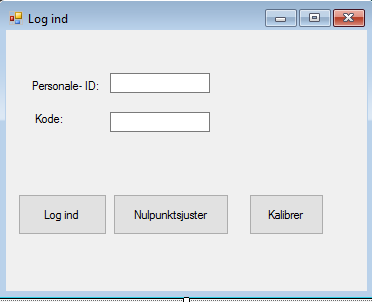
\includegraphics[width=0.7\textwidth]{Figurer/GUI/Logind_GUI}
	\caption{Login vindue}
	\label{Login vindue}
\end{figure}

I figur \ref{Login vindue} er der tage udgangspunkt i, at brugergrænsefalden skal være enkel og overskuelig opbygget. Der skal ikke være nogle overflødige ting og de knapper der er vigtige som bruger skal benytte skal stå tydeligt frem. Opbygningen skal afspejle brugerens logik.\\ \\ 
Tankerne omkring den enkle opbygning er, at hvis der opstår en akut situation hvor systemet skal i gang hurtigt skal det være nemt og hurtigt at logge ind i systemet. Det er vigtigt at knapperne er selvforklarende og giver brugeren det der forventes af knappen når den benyttes. \\ \\
Der er taget højde for feedback til bruger ved forkert log ind får brugeren en besked om at log ind er indtastet forkert og der skal prøves forfra. \\


\begin{figure}[H]
	\centering
	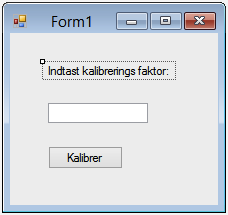
\includegraphics[width=0.7\textwidth]{Figurer/GUI/kalibrerGUI}
	\caption{Kalibrer vindue}
	\label{Kaliber vindue}
\end{figure}

Vist på figur \ref{Kaliber vindue}, hvor der her er lagt vægt på det funktionelle, med et enkelt og simpelt design. Der er vejledende tekst, som gør det nemt for aktøren at finde ud af systemet.

\begin{figure}[H]
	\centering
	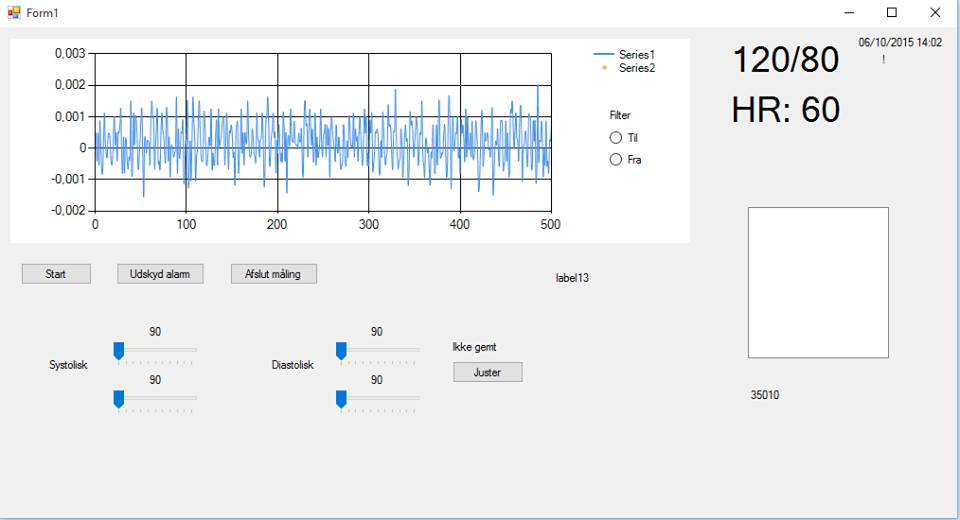
\includegraphics[width=1\textwidth]{Figurer/GUI/GUI_form1}
	\caption{Blodtryk vindue}
	\label{Blodtryk vindue}
\end{figure}

I blodtryksvinduet, vist på figur \ref{Blodtryk vindue}, er opbygningen mere kompliceret og med flere knapper end ved Log ind og Gem. Der er taget højde for at knapperne er selvforklarende og deres navne afspejler de bagvedliggende handlinger. Dette medfører at brugeren stadig har et overblik over brugergrænsefalden og stadig selv kan kontrollerer hvad der skal ske. Denne brugergrænseflade er ikke tiltænkt nye brugere, men derimod brugere der har et kendskab til den og til hvilke sundhedfaglige værdier og udtryk, der vises på den.  Derfor benyttes brugerens sprog på brugergrænsefalden og ikke et sprog med termer, der er forståelig for alle. 

\begin{figure}[H]
	\centering
	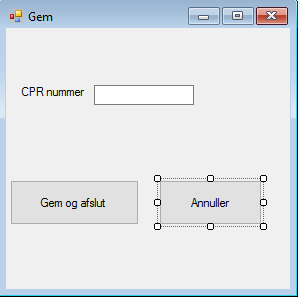
\includegraphics[width=0.7\textwidth]{Figurer/GUI/Gem_GUI}
	\caption{Gem vindue}
	\label{Gem vindue}
\end{figure}

På figur \ref{Gem vindue}, gemme-vinduet, er der igen taget udgangspunkt i en enkel opbygning og at knapperne, der skal bruges er tydelige og selvforklarende. Det er her også brugerens logik, der afspejles og ingen unødvendige ting er inddraget i brugergrænsefalden. Det er her muligt at afbryde situationen ved at der er en alternativ udvej, som kan bruges hvis den op startet handling fortrydes. Der er taget højde for feedback til brugeren hvis der indtastes forkert CPR nummer får brugeren det af vide i et pop-up vindue. 

\subsection{Domænemodel}
Diagrammet viser en domæne model for blodtryks systemet. Dette diagram giver et godt overblik over systemet som helhed og hvilke elementer, der indgår i systemet. Diagrammet viser hvordan brugeren interagerer med systemet og hvordan systemet forløber efter det igangsættes af bruger. 

\begin{figure}[H]
	\centering
	\includegraphics[width=1\textwidth]{Figurer/ISE/Domaenemodel}
	\caption{Domænemodel}
	\label{domaenemodel}
\end{figure}

\subsection{Appliktationsmodel}
Applikationsmodellen er en model der på baggrund af domænemodel og Use cases udarbejdes software relaterede klasse applikationsmodeller, sekvensdiagrammer og opdaterede klasse applikationsmodeller.\\
Her er det ikke-opdateret klassediagram udeladt, hvorfor sekvensdiagram og opdaterede  klasse applikationsmodel er udarbejdet på baggrund af fiktive metoder. De faktiske metoder kan ses i afsnit \ref{UML klassediagram}.

\subsubsection{Sekvensdiagram}
Sekvensdiagrammet er et interaktions diagram, der viser hvordan processer i systemet forløber. Use casene ligger til baggrund for udarbejdelsen af sekvensdiagrammerne.\\ \\
Der er blevet lavet et sekvensdiagram for hver use case for at give det bedste overblik over hver handling i forhold til systemet. I sekvensdiagrammet har vi brugt virtuelle metode kald til at beskrive forløbet. I use case 2-7 er det brugeren, der interagerer med systemet og er initiator for a handlingerne bliver udført.

\begin{figure}[H]
	\centering
	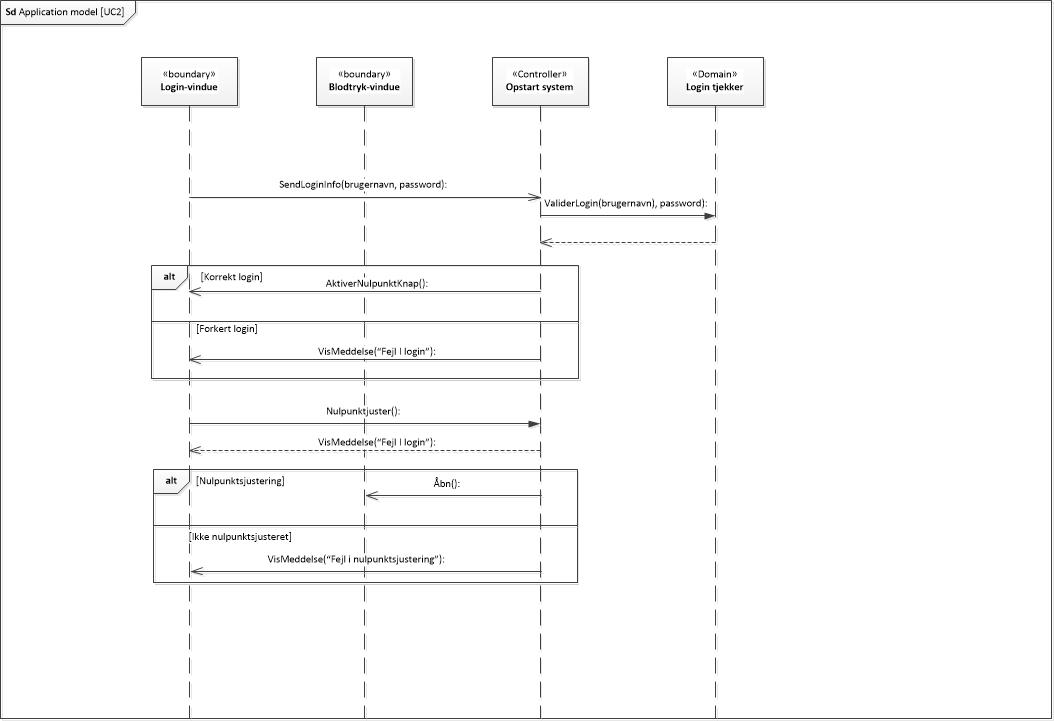
\includegraphics[width=1\textwidth]{Figurer/ISE/sdAppModelUC2}
	\caption{Sekvensdiagram UC2}
	\label{sd UC2}
\end{figure}

På figur \ref{sd UC2} ses det hvordan brugeren logger ind i systemet og hvordan brugeren for systemet nulpunktsjusteret. Det er brugeren, der interagerer med systemet og er initiator for at handlingerne bliver udført. 

\begin{figure}[H]
	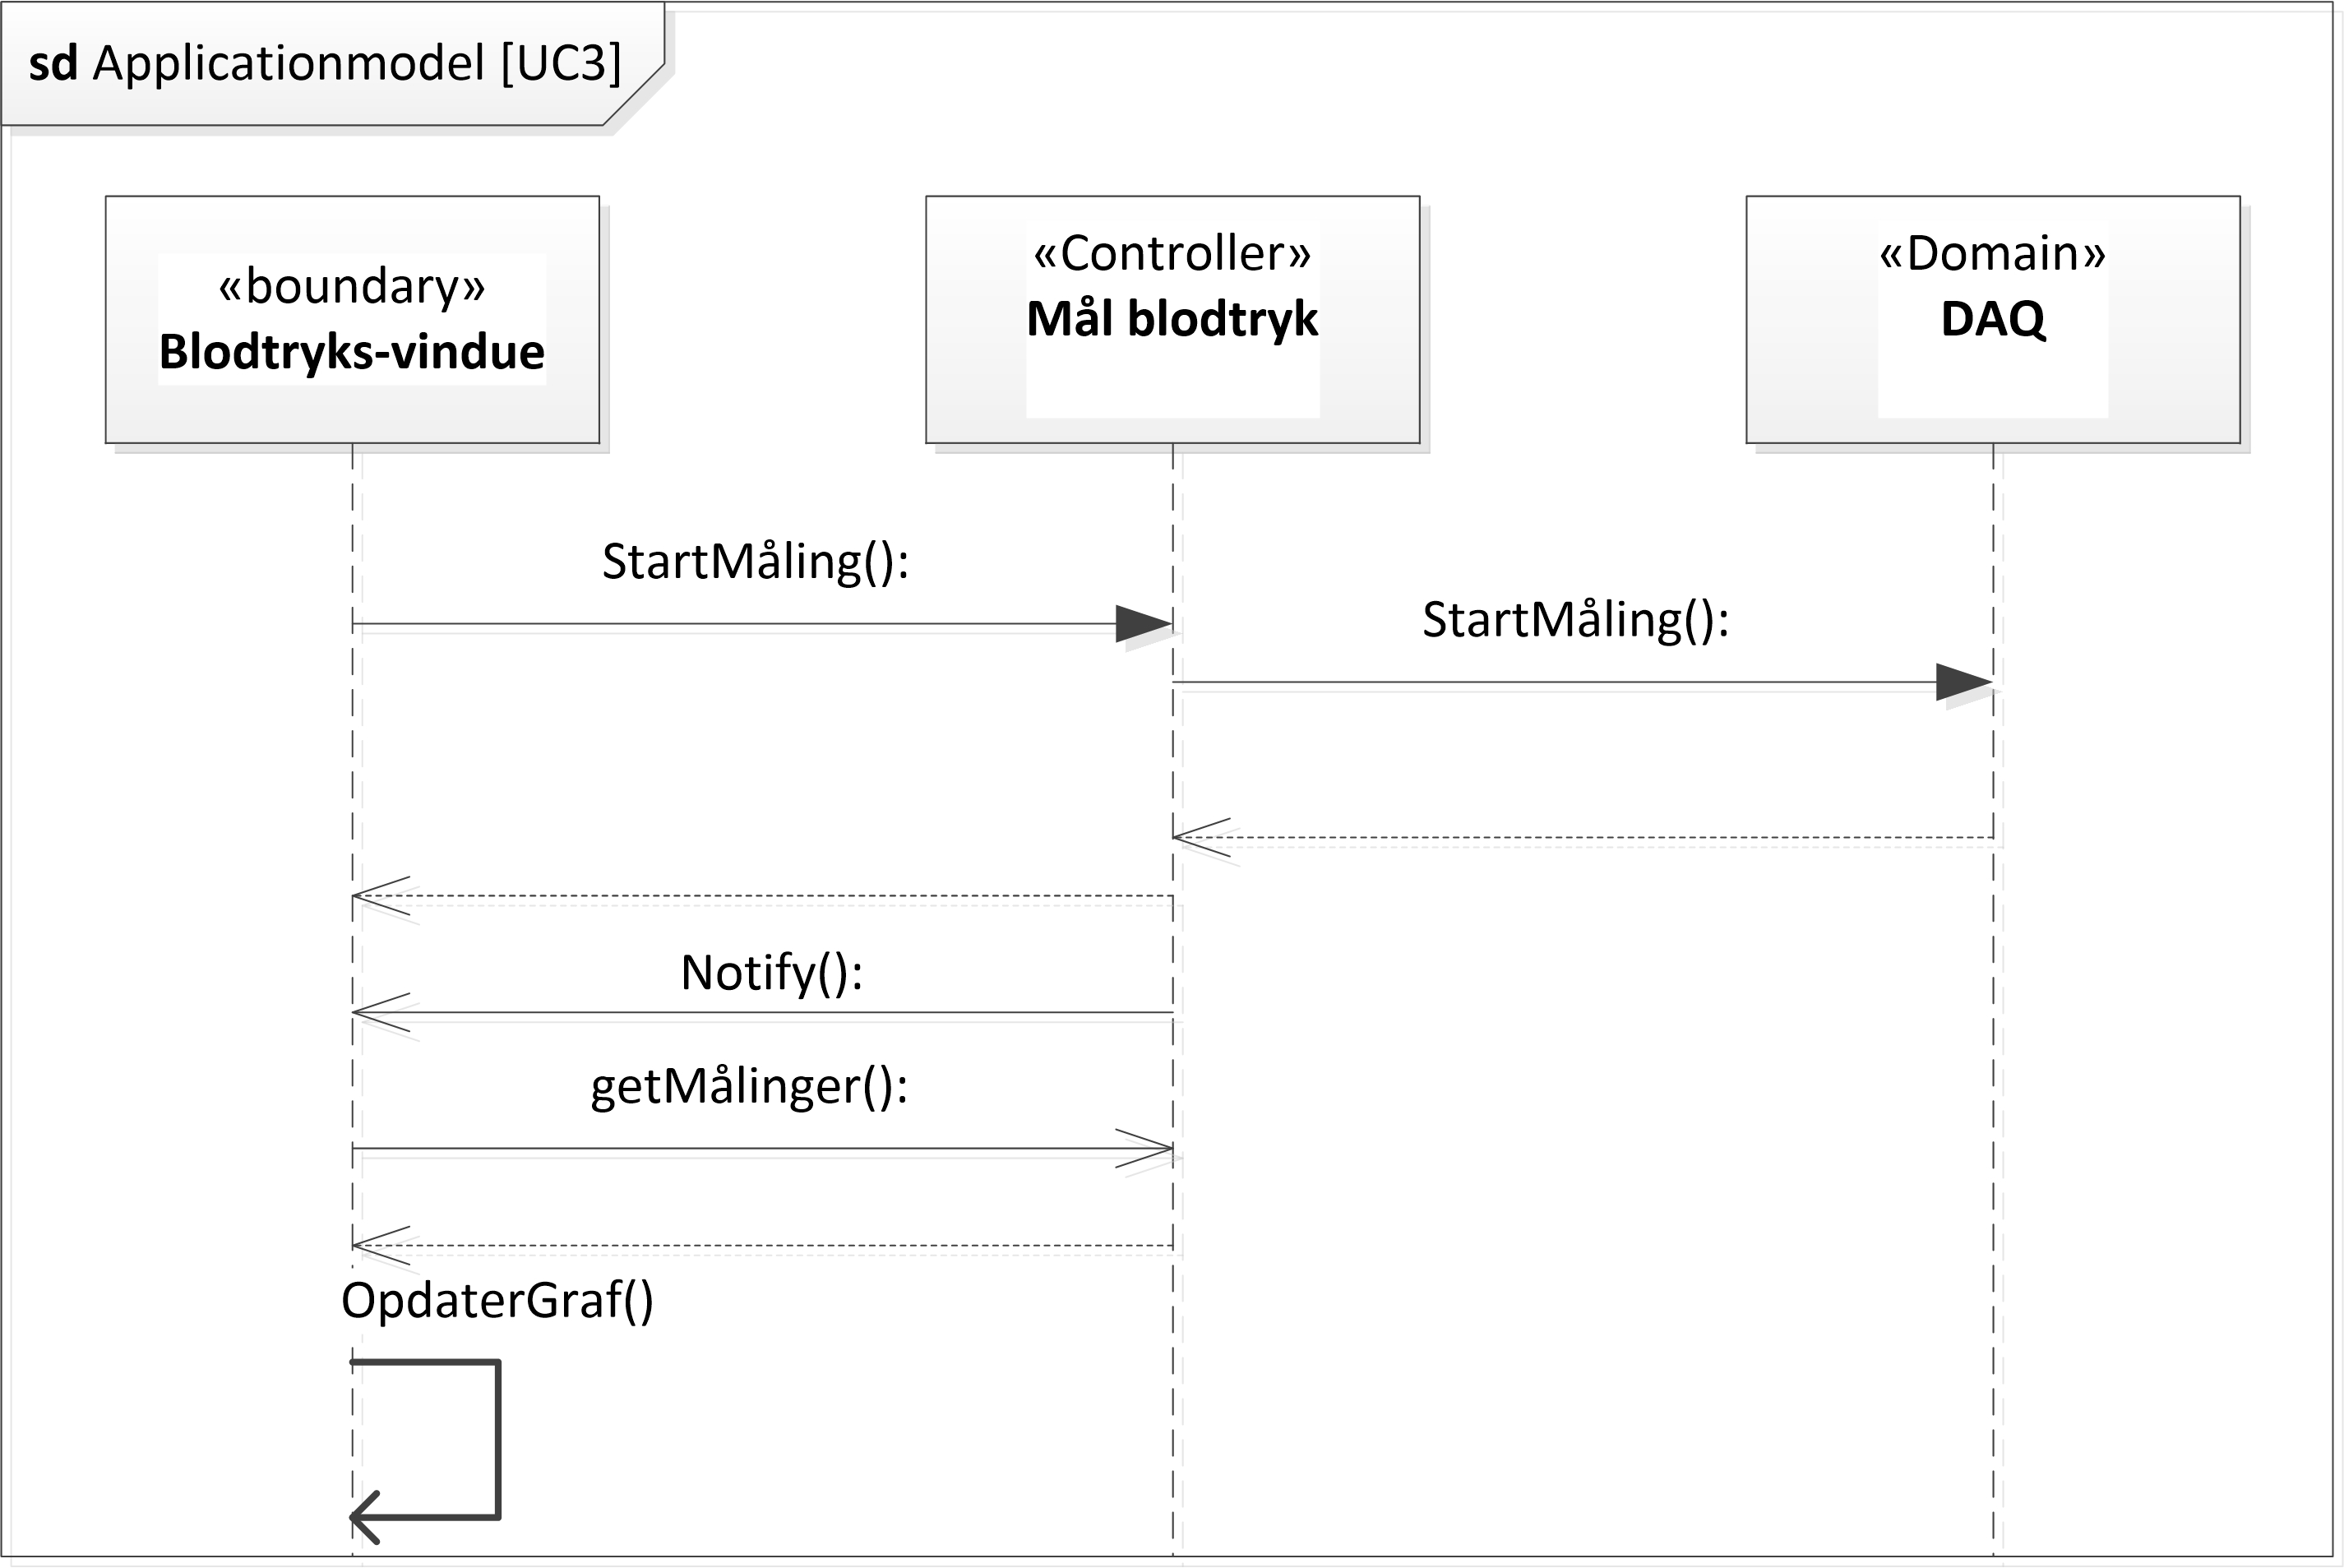
\includegraphics[width=1\textwidth]{Figurer/ISE/sdAppModelUC3}
	\caption{Sekvensdiagram UC3}
	\label{sd UC3}
\end{figure}

Figur \ref{sd UC3} viser hvordan brugeren starter målingen og hvordan graferne vises på brugergrænsefalden.

\begin{figure}[H]
	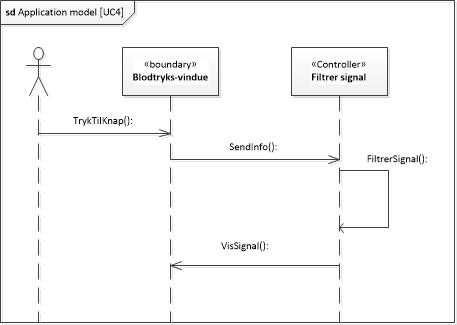
\includegraphics[width=1\textwidth]{Figurer/ISE/sdAppModelUC4}
	\caption{Sekvensdiagram UC4}
	\label{sd UC4}
\end{figure}

I sekvensdiagrammet figur \ref{sd UC4} ses hvordan brugeren kan vælge om blodtrykssignalet skal filtreres eller ej.

\begin{figure}[H]
	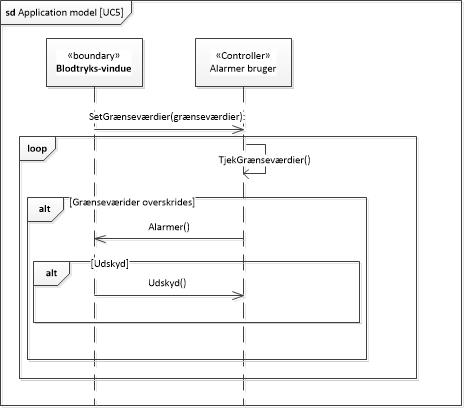
\includegraphics[width=1\textwidth]{Figurer/ISE/sdAppModelUC5}
	\caption{Sekvensdiagram UC5}
	\label{sd UC5}
\end{figure}

Det ses på figur \ref{sd UC5} hvordan brugeren justerer grænseværdierne for patientens blodtryk. Denne justering sker ud fra patientens målte blodtryk. De justerede grænseværdi ligger til grundlag for alarmen. Desuden viser figuren, at brugeren har mulighed for at udskyde alarmen.

\begin{figure}[H]
	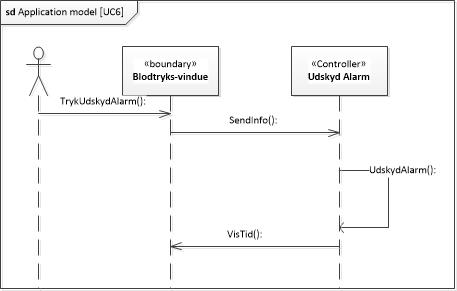
\includegraphics[width=1\textwidth]{Figurer/ISE/sdAppModelUC6}
	\caption{Sekvensdiagram UC6}
	\label{sd UC6}
\end{figure}

Figur \ref{sd UC6} viser hvordan systemet gemmer og afslutter en måling. 

\subsubsection{Opdateret applikationsmodel}
Klasse applikationsmodellerne er udarbejdet ud fra use casene, sekvensdiagrammer og domænemodellen. Der er ligesom ved sekvensdiagrammerne lavet et klassediagram for hver use case. Der er her også brugt virtuelle metoder. 

\begin{figure}[H]
	\centering
	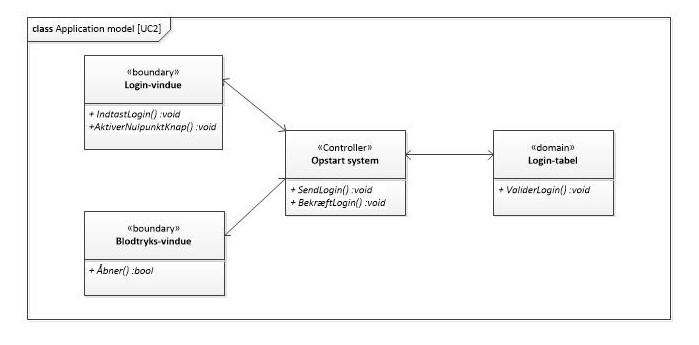
\includegraphics[width=1\textwidth]{Figurer/ISE/classAppModelUC2}
	\caption{Klassediagram UC 2}
	\label{classApp UC2}
\end{figure}

\begin{figure}[H]
	\centering
	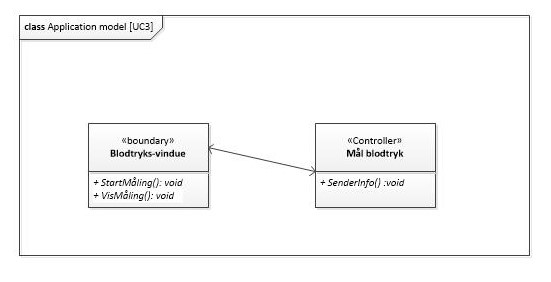
\includegraphics[width=1\textwidth]{Figurer/ISE/classAppModelUC3}
	\caption{Klassediagram UC 3}
	\label{classApp UC3}
\end{figure}

\begin{figure}[H]
	\centering
	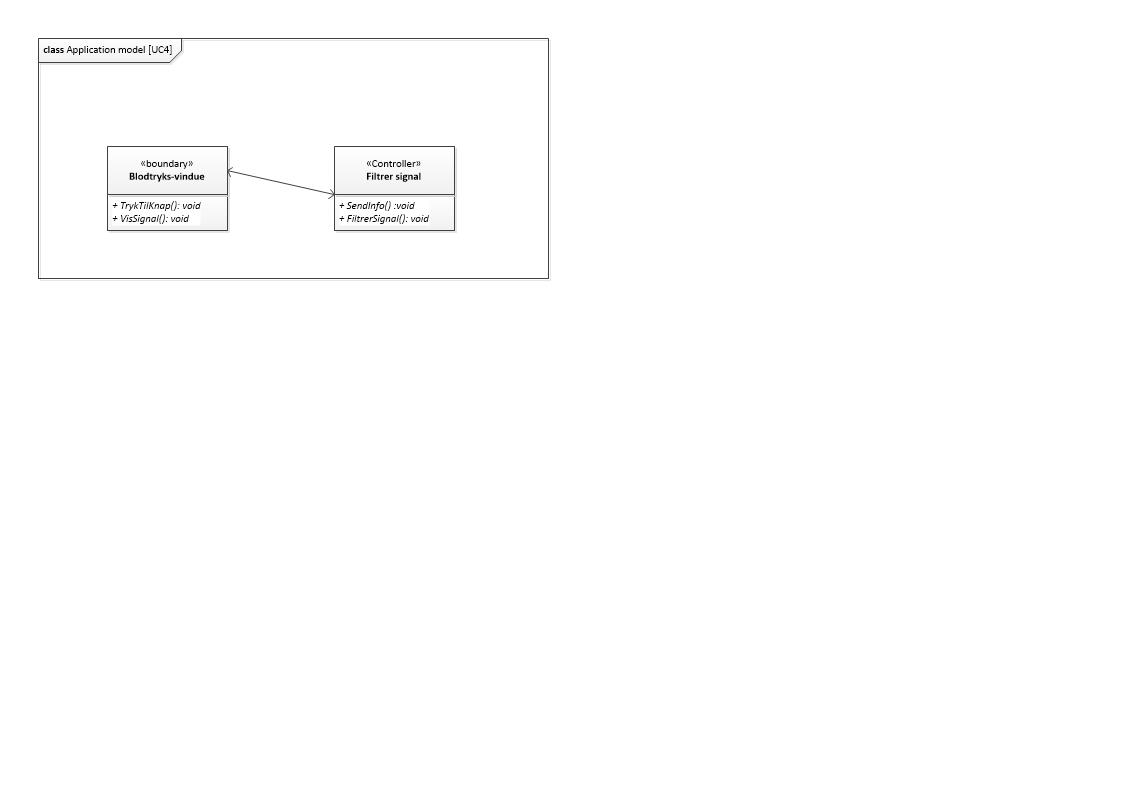
\includegraphics[width=1\textwidth]{Figurer/ISE/classAppModelUC4}
	\caption{Klassediagram UC 4}
	\label{classApp UC4}
\end{figure}

\begin{figure}[H]
	\centering
	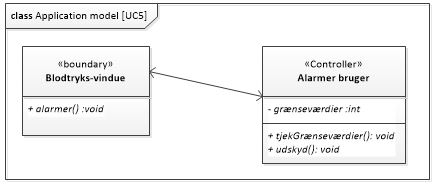
\includegraphics[width=1\textwidth]{Figurer/ISE/classAppModelUC5}
	\caption{Klassediagram UC 5}
	\label{classApp UC5}
\end{figure}

\begin{figure}[H]
	\centering
	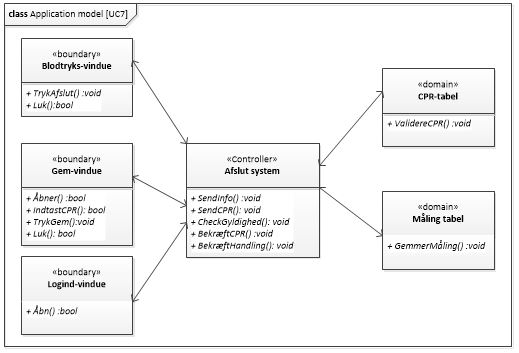
\includegraphics[width=1\textwidth]{Figurer/ISE/classAppModelUC7}
	\caption{Klassediagram UC 7}
	\label{classApp UC7}
\end{figure}

\chapter{Implementering}

\section{Hardware implementering}\label{Hardware implementering}

Efter teorifasen var ovre, blev de to blokke bygget op. Gruppen valgte at bygge forstærkeren og filteret på hver sit fumlebræt, dels på grund af pladsmangel og dels på grund af større sammenhæng mellem arkitekturen, og det endelige produkt.\\

\begin{figure}[H]
	\centering
	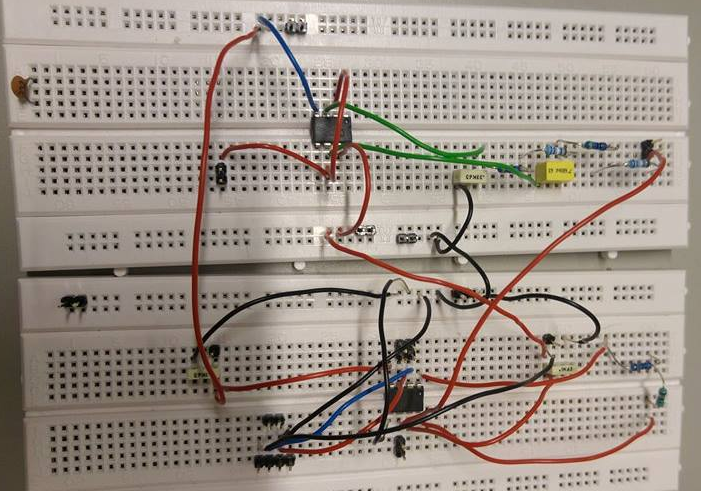
\includegraphics[width=1\textwidth]{Figurer/Hardware/samletopstilling}
	\caption{Opstilling af forstærker og filter}
	\label{Dsamletopbygning}
\end{figure}

Grundet mangel på præcise modstande, bedømte gruppen at det var bedst at bygge modstandende i forholdsvist filteret og forstærkeren, op i to, så gruppen kunne komme så tæt på den ønskede modstandsværdi som muligt. \\

\subsubsection{Hardware overvejelser}

I udviklingen af hardwaren, stødte gruppen på problematikker, som blev gjorde, at der var nogen komponenter, der blev nødt til at blive taget op til genovervejelse.\\
\\
Et af de største problemer gruppen stødte ind i, i forhold til hardware, var brugen af en operationsforstærker i forstærkerblokken. En reel operationsforstærker har ikke en uendelig indgangs modstand, som i den ideelle verden, og der er derfor en risiko for at den lave spænding fra transduceren simpelthen ikke ville kunne passere forstærkeren. Gruppen valgte derfor at bruge en instrumenteringsforstærker i stedet, da den reelle komponents egenskaber ligger langt tættere på dens ideelle modpart, og derfor var bedre egnet i gruppens kredsløb. En anden fordel ved instrumenteringsforstærkeren er, at den er meget let at justere gain på.\\
\\
En anden stor fordel ved instrumenteringsforstærkeren er, at common mode rejection er meget god. Common mode noise er støj, fra det omkringliggende miljø. Da en instrumenteringsforstærkers forstærkning kommer fra forskellen mellem dens to indgange, så kan støj påvirke forstærkningen, især når der arbejdes med så lave forstærkninger, som dem, der kommer fra transduceren. Ofte er der dog støj på begge indgange, og i den ideelle verden ville dette ikke påvirke forstærkningen. I den reelle verden kan støjen dog også ende med at blive forstærket. Common mode rejection beskriver hvor god en komponent er, til at sortere dette støj fra. Den brugte instrumenteringsforstærker har en common mode rejection på 120 dB, hvilket vurderes til en rimelig værdi. \\
\\
En anden ting ved forstærkeren, som blev nødt til at blive ændret, var det dynamik område, som skulle udnyttes. Oprindeligt havde gruppen bestemt, at det filtrerede signal skulle ligge imellem -5V til +5V. Grundet en forstærkers manglende evne til at forstærke et signal op til dens forsyningsspænding, så blev gruppen nødt til at nedsætte signalområdet til -2,5V til +2,5V. Det var muligt at forstærke signalet ydereligere, men grænsen blev sat til denne værdi, fordi signalområdet matcher et dynamikområde på AD konverteren.\\ 
\\
Designet af filteret, lå fast på forhånd, og der var derfor ikke meget der kunne ændres i dette. Operationsforstærkeren var oplyst til at skulle være af typen OP27G, da denne ligeledes har en god common mode rejection. Grundet mangel på præcise komponenter, har gruppen sat to modstande i serie, for at komme så tæt på den udregnede værdi, som muligt. \\
\\
Gruppen valgte desuden at systemet skulle forsynes af Analog Discovery, frem for et batteri. Dette skyldes at Analog Discovery giver en stabil strøm, som ikke har brug for at blive afbalanceret af en spændingsudligner. Gruppen vurderede at usikkerhederne ville udligne hinanden, og så flere fordele ved at bruge Analog Discovery.\\


\subsubsection{Implementering af forstærkeren}
Den samlede stykliste for forstærkeren blev vist som på tabel \ref{DForsttabel}.

\begin{table}[H]
\centering
\begin{tabular}{|l|l|l|ll}
\cline{1-3}
\textbf{Komponent} & \textbf{Antal} & \textbf{Type}  &  &  \\ \cline{1-3}
Modstand           & 1              & 120 $\Omega$   &  &  \\ \cline{1-3}
Modstand           & 1              & 4.8 $\Omega$   &  &  \\ \cline{1-3}
Kondensator        & 2              & 100 nF         &  &  \\ \cline{1-3}
Instrumentationsforstærker &    1   & INA114		     &  &  \\ \cline{1-3}
\end{tabular}
\caption{Forstærkertabel}
\label{DForsttabel}
\end{table}

For forstærkeren gælder det at den beregnede R$_{gain}$ er 125,31$\Omega$ som det kan ses ud af komponentlisten består R$_{gain}$ i praksis af to modstande på henholdsvis 4,8$\Omega$ og 120$\Omega$ som er sat i serie. R$_{gain}$ modstanden er i praksis 124,8$\Omega$. I praksis er R$_{gain}$ 0,51$\Omega$ mindre end den i teorien skulle have været.

\subsubsection{Implementering af filteret}
Den samlede stykliste for filteret blev som vist på tabel \ref{DFiltertabel}.

\begin{table}[H]
\centering
\begin{tabular}{|l|l|l|ll}
\cline{1-3}
\textbf{Komponent} & \textbf{Antal} & \textbf{Type}  &  &  \\ \cline{1-3}
Modstand           & 2              & 6.2 k $\Omega$ &  &  \\ \cline{1-3}
Modstand           & 2              & 470 $\Omega$   &  &  \\ \cline{1-3}
Kondensator        & 1              & 680 nF         &  &  \\ \cline{1-3}
Kondensator        & 1              & 330 nF         &  &  \\ \cline{1-3}
Operationsforstærker &    1         & OP27G          &  &  \\ \cline{1-3}
\end{tabular}
\caption{Filtertabel}
\label{DFiltertabel}
\end{table}

Det analoge filter består blandt andet af en 330 nF kondensator, C$_1$, som i teorien er beregnet til at skulle have været 333,2 nF. I praksis er kondensatoren C$_1$ 3,2 nF mindre end den i teorien er beregnet til at skulle have været. Filteret består desuden af to modstande R$_1$ og R$_2$ som er identiske. I det realiserede analoge filter består hver modstand af to modstande på henholdsvis 6200$\Omega$ og 470$\Omega$ som er sat i serie. Dermed er både R$_1$ og R$_2$ 6670$\Omega$ i praksis. I teorien var R$_1$ og R$_2$ udregnet til at skulle være 6687$\Omega$. I praksis er der derfor 17$\Omega$ mindre end teorien foreskriver.\\

Generelt er der valgt at se bort fra de afvigelser, der er for komponentværdierne i praksis sammenlignet med de i teorien beregnet. Det er valgt da afvigelserne er relativt små i forhold til det pågældende komponent. For modstandende er der desuden 1 procents usikkerhed, hvilket betyder man alligevel ikke kan være helt sikker på komponentværdien.\\

På baggrund af de i praksis anvendte komponenter er den reelle knækfrekvens for det analoge filter beregnet. Til det formål er formlen som set på figur \ref{dcutoff]} anvendt.\\

\begin{align}
f_{c} = \frac{1}{2\pi \sqrt{R_{1}C_{1}R_{2}C_{2}}} = \frac{1}{2\pi \sqrt{6687 \cdot 333,2\times 10^{-9} \cdot 6687 \cdot 680\times 10^{-9}}} = 50,37 Hz
	\label{dcutoff}
\end{align}

Desuden er den reelle $\zeta$ for dette filter, ifølge Okawadenshi, 0,697.


\section{Software implementering}\label{implementering}
Implementerings afsnittet beskriver hvilke faktiske handlinger der er foretaget ud fra arkitektur og design afsnittet. Yderligere beskriver afsnittet hvilke software orienterede metoder der er benyttet for at løse problemstillingen.

\subsection{3-lagsmodellen}
Softwaren er implementeret først og fremmest ud fra 3-lagsmodellen
3-lagsmodellen er bestående af lagene præsentationslag, logiklag og datalag.
Denne opdeling af lagene gør det langt lettere at vedligeholde systemet fordi der kan ændres i et enkelt lag uden det har indflydelse på resten af programmet. \\
Det er desuden en god software arkitektur at bruge ved et system udarbejdet af en gruppe, da der kan arbejdes på to forskellige lag af to personer samtidigt, hvis bare grænsefladerne bliver overholdt. 3-lagsmodellen er bygget op som vist på figur \ref{3lag}:

\begin{figure}[H]
	\centering
	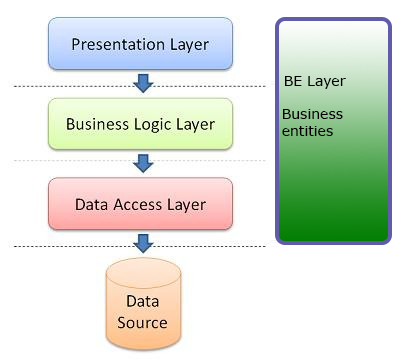
\includegraphics[width=0.8\textwidth]{Figurer/SoftwareImplementering/3lag}
	\caption{3-lagsmodellen}
	\label{3lag}
\end{figure}

\subsubsection{Præsentationslag}\label{praesentationslag}

Som vist på figur \ref{3lag}, er blodtrykssystemet bygget op med først et præsentationslag bestående af tre brugergrænseflader, som brugeren kan interagere med.\\
Login brugergrænseflade, bestående af tekstbokse til brugernavn og kodeord, samt paneler til både kalibrering og nulpunktsjusteringen, som vist på figur \ref{LoginGUI}:

\begin{figure}[H]
	\centering
	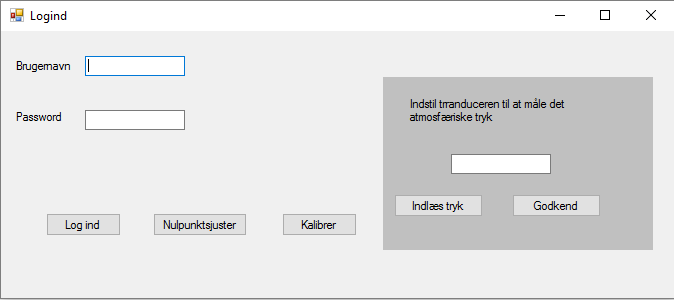
\includegraphics[width=1\textwidth]{Figurer/SoftwareImplementering/Logind}
	\caption{Login GUI}
	\label{LoginGUI}
\end{figure}
Dernæst åbnes hoved brugergrænsefladen, hvor blodtrykssignalet vises grafisk, samt brugeren har mulighed for at benytte en række funktioner i form af knapper og trackbars, som set på figur \ref{form1}

%\begin{figure}[H]
%	\centering
%	\includegraphics[width=1\textwidth]{Figurer/SoftwareImplementering/form1}
%	\caption{Blodtrykssystem hoved brugergrænseflade}
%	\label{form1}
%\end{figure}

Til sidst vises en brugergrænseflade for gemmefunktionen, hvor brugeren skal indtaste et CPR-nummer, samt bekræfte afslutning af målingen, se figur \ref{Gem}:

\begin{figure}[H]
	\centering
	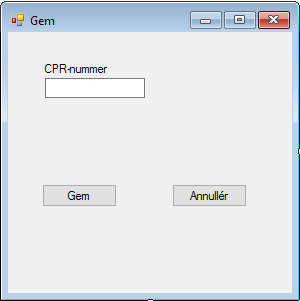
\includegraphics[width=0.6\textwidth]{Figurer/SoftwareImplementering/Gem}
	\caption{Gem GUI}
	\label{Gem}
\end{figure}

\subsubsection{Logiklag}\label{Logiklag}
Logik laget er det lag der spiller sammen med både data- og præsentationslag. Sammenspillet med præsentationslaget fungerer ved alt brugerens interaktion med systemet bearbejdes i logiklaget. Et eksempel herpå er det digitale filter, hvor brugeren gennem brugergrænsefladen tilslutter filteret. Dette igangsætter en metode i logik laget, som sørger for at signalet filtreres. Metoden er vist i figur \ref{filtrer} og figur \ref{Filtrer}:

\begin{figure}[H]
	\centering
	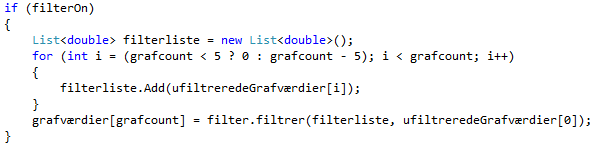
\includegraphics[width=1.15\textwidth]{Figurer/SoftwareImplementering/Filtrer1}
	\caption{Filtrer i filter klassen}
	\label{Filtrer}
\end{figure}

\begin{figure}[H]
	\centering
	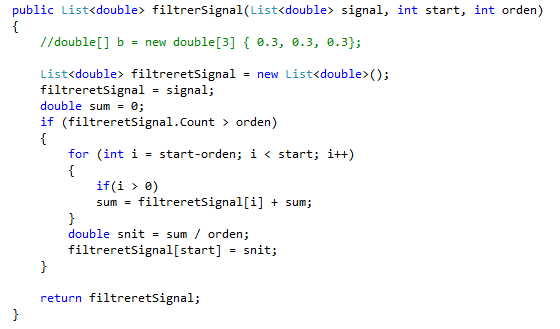
\includegraphics[width=0.85\textwidth]{Figurer/SoftwareImplementering/filtrer}
	\caption{Filtrer i filter klassen}
	\label{filtrer}
\end{figure}

Figur \ref{Filtrer} viser hvordan der i logikklassen oprettes en liste med .... \textbf{JEPPE!!!!}\\
Herefter bliver der i figur \ref{filtrer} taget gennemsnit af listen hvorefter den sidste værdi returneres, og derefter udskrives. Filteret er deraf et FIR filter af typen moving average.

\subsubsection{Datalag}\label{Datalag}
Datalaget er det lag som spiller sammen med databasen og logiklaget. Dvs. at datalaget modtager bruger inputs fra brugergrænsefladen gennem logiklaget. Herefter sender og validerer datalaget informationerne i en database. Eksempelvis er bliver login oplysninger tjekket i databasen via datalaget, dette er vist i figur \ref{Datalogin}:

\begin{figure}[H]
	\centering
	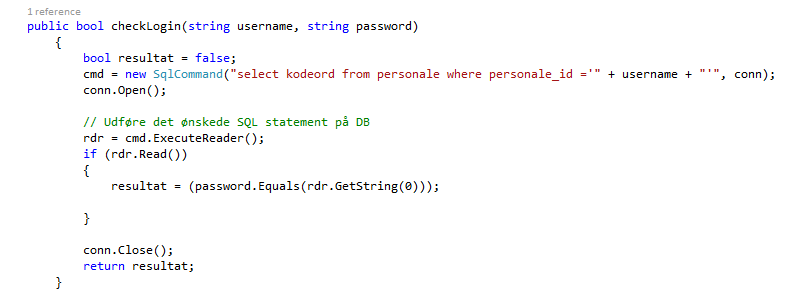
\includegraphics[width=1.4\textwidth]{Figurer/SoftwareImplementering/CheckLogind}
	\caption{Login tjekker metode}
	\label{Datalogin}
\end{figure}

Figur \ref{Datalogin} viser hvordan login tjekker metoden opretter forbindelse til en lokal database, hvorefter de indtastede værdier tjekkes i databasen. Til slut lukkes forbindelsen igen. Værdierne der tjekkes efter med kan ses i personale tabellen i databasen, som vist i figur \ref{personaletabel}

\begin{figure}[H]
	\centering
	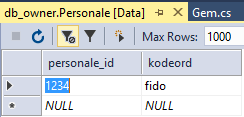
\includegraphics[width=0.6\textwidth]{Figurer/SoftwareImplementering/database}
	\caption{Personale tabel}
	\label{personaletabel}
\end{figure}

\subsection{Tråde}
Tråd programmering benyttes, når man som her ønsker flere opgaver i programmet udført løbende. Dette kan gør sig gældende eksempelvis ved at programmet ønsker at indlæse data og vise det i en graf, samtidig med at brugeren har adgang til alle interfacets funktioner. Det er disse delprocesser, som udgøre trådene. Hvis en enkelt tråd skulle gå i stå, skal de andre tråde stadig køre, således at programmet stadig kører videre. 
\subsection{Observer}
\subsection{Push pull}


\subsection{UML klassediagram}\label{UML klassediagram}


 







